%        File: lickly_hw3.tex
%      Author: Ben Lickly
%
\documentclass{article}
\title{EECS 219C: HW \#3}
\author{Ben Lickly}
\date{November 16, 2009}

\usepackage{amsmath}
\usepackage{amsthm}
\usepackage{algorithm2e}
\usepackage{graphicx}

\begin{document}
\maketitle
\begin{enumerate}
\item Express the following in LTL
  \begin{enumerate}
    \item \[G \left( (\neg p \wedge X p) \implies XG \neg (\neg p \wedge X p) \right) \]
    \item \[ GF (\neg p \wedge X p) \]
    \item \[ r \wedge G ( \neg ( r \wedge y \vee y \wedge g \vee g \wedge r)
      \wedge (r \implies X r \vee X g) \wedge (g \implies X g \vee X y)
      \wedge (y \implies X y \vee X r) ) \]
    \item \[G (q \implies X (\neg p U r)\]
  \end{enumerate}
\item LTL, CTL, CTL$^*$
  \begin{enumerate}
    \item This state machine does not satisfy the CTL formula because there exists an infinite path (namely the one that always stays in the leftmost blue state), for which there exists at every state a path that includes a state for which $p$ does not hold (namely the path that travels to the right).

      Claim: Any system that satisfies the CTL formula also satisfies the LTL formula.
\begin{proof}
  Assume that we have a system $S$ that satisfies $AF AG p$.  Let $z$ be an arbitrary path in the infinite computation tree of $S$.  Since we know that $F AG p$ holds for all paths in $S$, it also must hold for $z$.  Now let us consider the future state in $z$, call it $sf$, for which $AG p$ holds.  We know that all paths originating from $sf$ have the property $G p$.  In particular, so does the path that coincides with $z$.  Thus the entire path $z$ satisfies $FG p$, with the future state being $sf$.
\end{proof}
\item
$E(GF p)$ is not equivalent to $EG(EF p)$ because the first is a stronger restriction.  For example, take the Kripke structure in Figure~\ref{fig:p2b1}. This system has the property that $EG(EF q)$ since the path that stays in state $a$ will always have a future path that contains $q$.  On the other hand, there is no path for which $q$ is always true in the future ($E(GF p)$).
\begin{figure}
  \begin{center}
    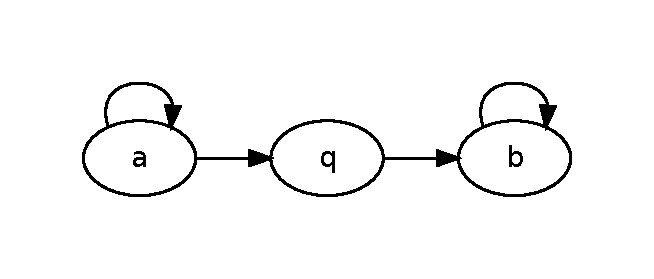
\includegraphics[scale=0.5]{p2b1}
  \end{center}
  \caption{Example distinguishing $E(GF p)$ from $EG(EF p)$}
  \label{fig:p2b1}
\end{figure}

  $E(GF p)$ is not equivalent to $EG(AF p)$ because the second is a stronger restriction. For example, take the Kripke structure in Figure~\ref{fig:p2b2}.  Here, there exists a path in which $q$ is always true in the future ($E(GF q)$), namely the path that switches between $a$ and $q$.  On the other hand, it is not true that $EG(AF q)$, since no matter what path we choose, there always will exist some branching path that stay forever in $a$.
\begin{figure}
  \begin{center}
    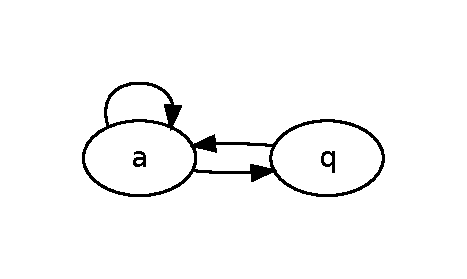
\includegraphics[scale=0.5]{p2b2}
  \end{center}
  \caption{Example distinguishing $E(GF p)$ from $EG(AF p)$}
  \label{fig:p2b2}
\end{figure}
\item
\begin{enumerate}
  \item These two CTL formulas are equivalent. There exist a path that has one of two properties true in the future if and only if there exists a path that has one true or the other.
  \item These are not equivalent.  A computation tree that distinguishes them is given in Figure~\ref{fig:p2c}.  Here it is not the case that either $AFp$ or $AFq$, but it is true that $AF(p \vee q)$.
\begin{figure}
  \begin{center}
    \includegraphics[scale=0.5]{p2c}
  \end{center}
  \caption{Example distinguishing $(AF p) \vee (AF q)$ from $AF(p \vee q)$}
  \label{fig:p2c}
\end{figure}
\end{enumerate}
  \end{enumerate}
\item Fixpoint Characterization of $AFp$
  %FIXME: Review Chapter 6 of the Clarke et al. book

  Prove that the set of states satisfying $AF p$ is the least fixpoint of the function $\tau$ given by $\tau(Z) = p \vee AX Z$.

\begin{proof}
  Claim 1:  $AF p$ is a fixpoint of $\tau$.

  \[\tau(AF p) = p \vee AX(AF p) = p \vee X(AF p) = AF p \]
  Thus $AF p$ is a fixpoint of $\tau$.

  Claim 2: For any fixpoint of $\tau$ $S$, $AF p \supseteq S$.

  Assume to the contrary that this were not the case.  This would mean that
  there exists some computation $Z \in S$ such that $Z \not\in AF p$.
  This would mean that there exists a path for which $p$ is not true,
  or $EG \neg p$.  Now if we take $\tau(Z)$, we get $p \vee AX(EG \neg p)$,
  which is clearly not equivalent.  Thus $S$ is not a fixed-point of $\tau$.
  This contradicts our assumption.
\end{proof}

\item Simulation and SAT
  \begin{enumerate}
    \item How many boolean variables do we have?
      \[ |S| \times |S'| \]
    \item Suppose that two states $s$ and $s'$ have the same label. \dots

      In general, the CNF clause will be of the form:
      \[ \neg x_{s,t} \vee x_{s',t'_1} \vee \dots \vee x_{s',t'_k} \]

      In the case where there are no successors of $s'$, this simplifies to:
      \[ \neg x_{s,t} \]

      Clearly, there can be no more of these clauses than there are boolean
      variables. i.e. $|S| \times |S'|$
    \item
      \[ x_{s_0,t'_1} \vee \dots \vee x_{s',t'_k} \]
      where $t'_k \in S'_0$
    \item The overall problem is isomorphic to a Horn-SAT problem
      (by simply negating all the boolean variables).  This means that there
      is an efficient algorithm to solve it since Horn-SAT takes time
      proportional to the number of literals in the problem.
  \end{enumerate}
\item Symmetry Reduction

  The Kripke structure in Figure~1 has two automorphisms, namely the identity
  function, and $f$ given as follows:
  \[
  f(x) = \begin{cases}
    s0 &\text{if } x = s1 \\
    s1 &\text{if } x = s0 \\
    s2 &\text{if } x = s3 \\
    s3 &\text{if } x = s2
  \end{cases}
  \]
  The orbits are $\left\{ s0, s1 \right\}$ and $\left\{ s2, s3 \right\}$.
\item SPINing Elevators
  \begin{enumerate}
    \item The elevator never moves with its doors open.

      \[ G (moving \implies \neg doors\_open )\]
      This is valid, no matter how many passengers there are.

    \item Whenever a user at floor 1 requests the elevator and it is not at
      floor 1, then it eventually arrives at that floor and opens its doors.

      \[ G ( \wedge_{p \in NP} waiting_floor0[p] \implies F \neg waiting_floor0[p] )\]
      This is true for one and two passengers, but is invalid for three.
      The counterexample is shown in Figure~\ref{fig:waiting3}.
      Here, because the channel for remembering button presses is only
      two units long, the third passenger's call to the lift is effectively
      forgotten.
\begin{figure}
  \begin{center}
    \includegraphics[scale=0.6]{waiting3}
  \end{center}
  \caption{Example in which third passenger cannot catch lift}
  \label{fig:waiting3}
\end{figure}

    \item The elevator visits every floor infinitely often.
      \[G \left( (F floor == 0) \wedge (F floor == 1)
      \wedge (F floor == 2) \wedge (F floor == 3) \right) \]
      Trying to verify this property produces a counterexample, where one
      user simply exits and enters the elevator at floor 0
      forever, with the elevator completely missing two floors
      and only spending an infinite amount of time at one floor.
      This is the case no matter how few passengers there are.
\begin{figure}
  \begin{center}
    \includegraphics[scale=0.6]{every_floor1}
  \end{center}
  \caption{Example in which all floors are not reached}
  \label{fig:everyf}
\end{figure}
  \end{enumerate}
\end{enumerate}

%\bibliographystyle{plain}
%\bibliography{lickly_hw1}
\end{document}

